\documentclass{book}

\counterwithin{figure}{section}

% General
\usepackage{setspace} % helps with spacing
\usepackage[toc]{appendix} % appendix
\usepackage{pdfpages}

% Graphics
\usepackage{graphicx} % Required for inserting images
\usepackage{caption}
\usepackage{subcaption}
\usepackage{tikz} % to draw graphics
\usepackage{matlab-prettifier} %matlab code
\usepackage{verbatim}

% Math
\usepackage{amsmath} % Apparently required for equation design
\usepackage{gensymb} % for the degree symbols
\usepackage{bm} % bold for greek letters
\usepackage{mathtools}
\usepackage{amssymb}
\usepackage{amsfonts}

%tikzpicture
\usepackage{tikz}
\usepackage{scalerel}
\usepackage{pict2e}
\usepackage{tkz-euclide}
\usepackage{circuitikz}
\usetikzlibrary{calc}
\usetikzlibrary{patterns,arrows}
\usetikzlibrary{shadows}
\usetikzlibrary{external}
\usetikzlibrary{positioning}
\usetikzlibrary{arrows.meta}
\usetikzlibrary{arrows, decorations.markings}
\tikzstyle{vecArrow} = [thick, decoration={markings,mark=at position
   1 with {\arrow[semithick]{open triangle 60}}},
   double distance=2pt, shorten >= 5.5pt,
   preaction = {decorate},
   postaction = {draw,line width=1pt, white,shorten >= 4.5pt}]
\tikzstyle{innerWhite} = [semithick, white,line width=1.4pt, shorten >= 4.5pt]

%pgfplots
\usepackage{pgfplots}
\pgfplotsset{compat=newest}
\usepgfplotslibrary{statistics}
\usepgfplotslibrary{fillbetween}

%colours
\usepackage{xcolor}

% References
\usepackage{todonotes}

% Subfiles
\usepackage{subfiles}

% Hyperlinks
\usepackage{hyperref, cleveref}
\hypersetup{%
    colorlinks=true,
    linkcolor=blue,
    citecolor=cyan,
    pdftitle={Thesis},
    pdfpagemode=FullScreen
}

% Geometry
\usepackage{setspace}

\usepackage{geometry}

\geometry{
a4paper,
left=25.4mm,
top=25.4mm,
right=25.4mm,
bottom=25.4mm
}

\doublespacing

% \title{Master's Thesis}
% \author{Oswald Lawson}
% \date{October 2024}

\begin{document}

\begin{titlepage}
    \begin{center}
        \vspace*{2cm}

        \LARGE
        \textbf{Working Title: Power Transfer Device}

        \vspace{0.5cm}
        \large
        Master's Thesis

        \vspace{1.5cm}
        
        \Large
        \textbf{Oswald Lawson}
        
        \vspace{0.5cm}

       \large
        251025323
        
        \vfill

        Faculty of Engineering

        \vspace{0.25cm}
        The University of Western Ontario

        \vspace{0.25cm}
        Department of Electrical and Computer Engineering

        \vspace{0.25cm}
        

        \vspace{0.25cm}
        \today
 
    \end{center}
\end{titlepage}

 \hypersetup{linkcolor=black} 
 \tableofcontents

\newpage

\chapter{Introduction} \label{Introduction}

\section{Motivations}
% \todo{Expand upon this section}
Reliable access to electricity is a critical component of a prosperous society. Increasing access to energy in areas that lack that access \cite{international2022world}. Furthermore, given that electricity is foundational to economic growth and the maintenance of social services like education and healthcare \cite{owid-sdgs-affordable-clean-energy}, people remain interested in maintaining and increasing energy production and distribution. 

\section{Microgrids} \label{Introduction:Microgrid}
Microgrids, which consist of power sources servicing loads, exchange around 10 MVA of power \cite{Uddin_Microgrid_Scale, Trends_in_Microgrid} Microgrids operate using either DC, single-phase AC, or three-phase AC electricity \cite{Uddin_Microgrid_Scale}. By contrast, nanogrids, or systems that provide electrical power to a single building or small cluster of buildings, can have individual power ratings of approximately 10 kVA \cite{Pindoriya_Nanogrid_Rating}. Nanogrids typically operate using DC or single-phase AC electricity \cite{Jie_Nanogrid_Rating, Pindoriya_Nanogrid_Rating}. 

\subsection{Three-Phase AC Microgrids}

Three-phase AC microgrids typically service small industrial loads.

\textcolor{blue}{
\begin{itemize}
    \item Typical load size
    \item Locations
    \item Configuration (diagram)
\end{itemize}
}

\section{Connections between two Microgrids}

The interface of a microgrid into a power system typically consists of power electronic-based systems \cite{Barnes}. Bidirectional power transfer across these systems is typically a feature \cite{Deng}. Research is being undertaken to improve stability of microgrids, which are often conceptualized as relatively “weak” systems \cite{Rezaee}.

\subsection{Issues in Microgrid Interconnections}
Issues in microgrid interconnections include the following:
\begin{itemize}
    \item Interconnection transients
    \item Power allocation (energy management)
    \item Rapid Dynamics (to a greater extent than a microgrid-grid interconnection)
    \item Response to faults and other voltage imbalances 
\end{itemize}

\section{Problem Statement}

Considering two islanded microgrids supplying residential or light industrial loads, the broad research question is to explore how interconnecting these microgrids can improve their operation.

To explore this question, a minial microgrid power system is defined as a generator of fixed rating powering a load that can vary in demand. The central problem is: if an interconnection is placed between two such power systems and the load demand on one of the generators exceeds the capacity of the generator powering it, how can excess capacity from the other power system be used to relieve the first one?

\section{Research Objectives}

\subsection{Project Scope}

For validation of prototypes like the one being proposed in this work, it is typical that a much smaller scale system is used. Typical power ratings of prototype back-to-back converters have ranged from 1.5 kVA to 5 kVA \cite{Wu_Model_Size, Jung_Model_Size} and have worked with source voltages around 208 V at frequencies of 50-60 Hz \cite{Blaabjerg_Grid_Synchronization, Wu_Model_Size, Jung_Model_Size}, indicating that prototypes of that size have generally been effective at demonstrating that proposed concepts are valid. Thus, the chosen power rating of this project’s bidirectional converter is 5 kVA, and source voltages will be of 208 V at 60 Hz, as shown in \autoref{fig:Quick_Abstraction}. 

\begin{figure}
    \centering
    \includegraphics[width=0.95\linewidth]{Images/Quick_Abstraction_2024.11.11.png}
    \caption{High-level Model with System Power Ratings}
    \label{fig:Quick_Abstraction}
\end{figure}

\section{Contributions}

\textcolor{blue}{
\begin{itemize}
    \item Interconnection design for weak microgrids of particular size
    \item Validation using real-life objects
    \item Validation using particular switching scheme
\end{itemize}
}

\section{Thesis Organization}

The rest of this thesis is organized as follows. Chapter 2 deals with the theory of synchronization between two power systems with individual frequency, phase, and voltage characteristics. Chapter 3 discusses theoretical bases for the interconnection of two three-phase power systems. Chapter 4 simulates a potential experimental set-up to evaluate a potential interconnection. Chapter 5 discusses the experimental set-up to evaluate a potential interconnection. Chapter 6 evaluates the results of that experimental setup and discusses the implications. Chapter 7 concludes the thesis and explores bases for future work.

\chapter{Literature Review}

\textcolor{blue}{
\begin{itemize}
    \item Synchronization of a Power Source to a Grid
    \item Describing a "strong" grid vs a "weak" grid (i.e., the difference between a centralized grid and a microgrid)
    \item Types of Interconnections between Two Microgrids
    \item Research Gaps: (e.g., Limited real-life implementations of simulated microgrid interconnections)
\end{itemize}
}

This chapter will discuss existing approaches that connect three-phase microgrids and identify research gaps.

% \section{Microgrid Interconnections}

% Microgrids can be connected in three ways.

\section{Microgrid Interconnection and Interconnection Approaches}

One possible strategy for the interconnection of two microgrids uses bidirectional power electronic converters \cite{Blaabjerg_Grid_Synchronization}. To ensure that a stable interconnection can be formed, each side of the interconnection must be synchronized to the microgrid at the terminal. To conduct this synchronization, the convention is to use the synchronous reference frame phase-locked loop (SRF-PLL) \cite{Guerrero_Vasquez_3PLL}.

\subsection{Synchronization Approaches}

When using power electronic converters to interface between power systems, it is necessary to ensure that the voltage, frequency and phase at the point of connection is synchronized. Several algorithms have been investigated for that purpose; they include, among others, the zero-crossing method and the phase-locked-loop \cite{Blaabjerg_Grid_Synchronization}. Individual power sources and loads can have significant influence on the system voltage and frequency of microgrids, making those especially prone to distortions.

\subsection{The Synchronous Reference Frame Phase-Locked-Loop}

\begin{figure}
    \centering
    \includegraphics[width=0.95\linewidth]{Images/PLL_Diagram_2024.11.11_OTL.png}
    \caption{A diagram of the PLL}
    \label{fig:PLLDiagram}
\end{figure}

Within a synchronous reference frame phase-locked-loop (SRF-PLL) are three components: the phase-detection mechanism, the loop filter, and the voltage-controlled oscillator (the VCO). \autoref{fig:PLLDiagram} shows the three components. $v_{abc}$ is the three-phase input voltage, $v_q$ is the quadrature voltage in the $dq$ representation of the input voltage, $\omega_n$ is the nominal grid frequency, and $\theta$ is the estimated grid phase. In three-phase SRF-PLLs, the phase detection mechanism accepts a three-phase signal, determines its phase, and compares it to the estimated phase signal.

The loop filter is generally a PI (proportional-integral) controller with control law

\begin{equation}
    \frac{k_p s + k_i}{s}
\end{equation}

Finally, it can proven that the VCO is an integrator \cite{Blaabjerg_Grid_Synchronization}. Literature has shown that the SRF-PLL is a second-order system (i.e., a system with two open-loop poles). Therefore, it can track a constant reference signal with zero steady-state error; however, it cannot track a ramp signal without steady state error \cite{Guerrero_Vasquez_3PLL}. 

\subsection{Synchronization between a Weak Microgrid and a Strong Grid}

Substantial research has been done on synchronization between a "small" grid or power system and a much larger one \cite{Blaabjerg_Grid_Synchronization, Blaabjerg_Microgrids_Control, Guerrero_Hierarchical}.

\subsection{Synchronization between Two Microgrids}

Some work has been done to analyze the interlinking of several microgrids. For example, \cite{Blaabjerg_Interlinking} considers the linking between a single-phase AC microgrid and a DC microgrid. 

The reference \cite{Blaabjerg_Microgrids_Control} discusses synchronization within the “weak” three-phase microgrid as being effected with two types of PLLs: either the SRF-PLL discussed within the previous section or a synchronous reference frame frequency locked loop (SRF-FLL). SRF-PLLs are said to work well when the grid with which to be synchronized has a balanced signal; in contrast, more advanced PLLs are required for signals that are distorted. In contrast, SRF-FLLs are said to be less responsive to phase-angle jumps in the synchronizing signal, making it more desirable in the event of a distorted signal. However, the SRF-FLL’s architecture is more complex than the SRF-PLL’s. 

\section{Research Gaps}

Potential research gaps exist in areas including synchronization quality and consideration of the use of more robust PLLs, and modulation schemes. For example, simulation data for an AC-DC power converter has shown that the SVPWM algorithm can be used in an effective manner to implement bidirectional power transfer \cite{Deng}. Simulation data shows that converters that make use of the SVPWM algorithm have more robust dynamic and steady-state response \cite{Wang}. Finally, with regards to DC-AC power conversion, the SVPWM algorithm makes greater use of available DC voltage in comparison to SPWM, another commonly used modulation scheme \cite{Zhang}.

\chapter{Theoretical Bases}

This section describes the mathematical modelling of the solution and discusses the technical scope of the project.

\textcolor{blue}{
\begin{itemize}
    \item Model of a Simple Microgrid (e.g., voltage source, current source)
    \item "Accurate" model of Power Electronic Converters
    \item Average Model of Power Electronic Converters
    \item Power transfer using droop control
\end{itemize}
}

\begin{comment}

\section{The Average Model of Power Electronic Converters}

Power electronic converters are operated by switching transistors at frequencies in kHz. This switching causes harmonics, which can cause complications in modelling and simulating the converters' behaviour. Average models can thus be used to simplify the description and simulation of the converters \cite{Jankovic_Averaged_Model}.

\section{Project Definitions} \label{Theoretical_Bases_Project_Scope}

(This section will be expanded upon). 

\end{comment}

\chapter{Investigation by Simulation}

\textcolor{blue}{
\begin{itemize}
    \item Simulated Microgrid
    \item Simulation of "accurate" interconnection model for 1-2 seconds using SPWM
    \item Simulation of "accurate" interconnection model for 1-2 seconds using SVPWM
    \item Simulation of averaged model of interconnection for longer durations (e.g., 1 minute)
    \item Simulation to demonstrate transfer of poweR 
\end{itemize}
}

\section{Model Simulation}

As has been described, the intent of this project is to form an interconnection via which two microgrid- and nanogrid-scale power systems can exchange power as needed. It is critical to identify key characteristics of these power systems.

\subsection{Three-Phase SRF-PLL}

For the purposes of this experiment, it has been decided that a phase-locked loop is to be used for synchronization; that is because it has a greater ability to withstand distortions within the input signal and disturbances at the output \cite{Guerrero_Vasquez_3PLL}.

A key component of the synchronizing module, the three-phase SRF-PLL, is modeled in \textsc{MATLAB}. To verify its ability to track a changing reference frequency, its response to the example input signal 
\begin{equation}
    u(t) = \sin(2{\pi}ft)
\end{equation}
is simulated. The value of $f$ in this signal varies from 60 Hz to 65 Hz.
\begin{comment}
\begin{figure}
    \centering
    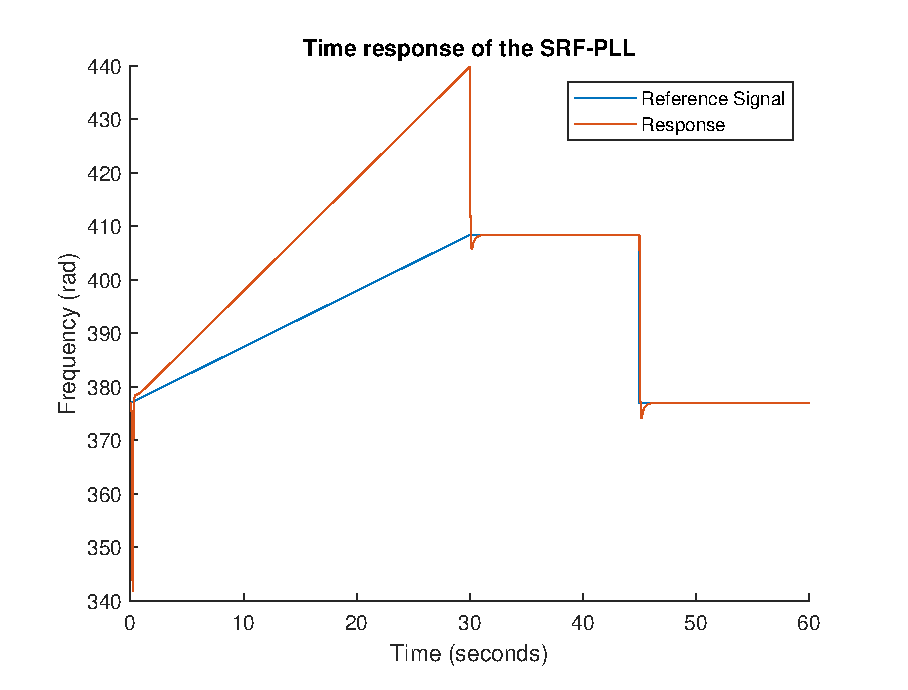
\includegraphics[width=0.75\linewidth]{Images/Sine_variation_Graph_Real.eps}
    \caption{The response of the simulated SRF-PLL}
    \label{fig:SRFPLL_Fig1}
\end{figure}
\end{comment}
The response is graphed in \autoref{fig:SRFPLL_Fig1}, The results show that, while the SRF-PLL cannot track a ramp signal without steady-state error, it is able to track a constant signal.

To test the PLL's response within the context of a power system, its performance in measuring an inverter's output frequency is tested. The simulation environment within MATLAB is shown in \autoref{fig:SimInverter}. The inverter is powered by a DC voltage source at 208 $V$. The PLL has proportional gain $k_p = 2$ and integral gain $k_i = 1000$. The reference signal is

\begin{equation*}
    \textbf{u}(t) = 
        \begin{bmatrix}
            120\sin(377t) \\
            120\sin(377t - \frac{2\pi}{3}) \\
            120\sin(377t - \frac{4\pi}{3})
        \end{bmatrix} \mathrm{V}
\end{equation*}

which is a three-phase signal with frequency of 60 Hz. It assumed to come from an infinite bus. 

\begin{figure}
    \centering
    \includegraphics[width=\linewidth]{Images/MATLAB System.png}
    \caption{Simulated Inverter}
    \label{fig:SimInverter}
\end{figure}

The graph in \autoref{fig:SimInverter_Frequencies} shows that, while there is substantial overshoot, the response is extremely rapid, settling to its final value of 60 Hz in less than 0.2 s. This suggests that the designed PLL can track changes in reference frequencies, but it may risk reacting too quickly to noise from a reference signal.

\begin{figure}
    \centering
    \includegraphics[width=0.95\linewidth]{Images/Frequencies.eps}
    \caption{Output Frequencies of Simulated Inverter}
    \label{fig:SimInverter_Frequencies}
\end{figure}

\subsection{Model of the "Weak" Power Systems}

\subsection{Model of a Power Electronic Based Bidirectional Converter}

As a baseline, an AC-AC converter with a DC link is simulated. The AC-AC converter is composed of two six-switch converters (i.e., a rectifier and an inverter) in cascade. In simulation, the terminals of both six-switch converters are connected to a three-phase voltage source and a three-phase load, respectively, to evaluate whether both terminals could serve in each capacity. Furthermore, to ensure that both terminals can service power sources and/or loads that are serving at different frequencies, each terminal is tested with a 60 Hz power source and a 50 Hz load. The results are plotted below. It can be seen that, on both ends, the desired frequencies are obtained.

\begin{figure}[h]
    \centering
    \includegraphics[width=0.6\linewidth]{Images/IMG_0994.png}
    \caption{Frequency of Power Source in Simulated AC-AC Converter}
    \label{fig:Investigations_60Hz}
\end{figure}

The image in \autoref{fig:Investigations_60Hz} shows the frequency of the input fixed voltage source. It is 60 Hz. Meanwhile, the image in \autoref{fig:Investigations_50Hz} shows the frequency at the load-side terminal. It is 50 Hz.

\begin{figure}[h]
    \centering
    \includegraphics[width=0.6\linewidth]{Images/IMG_0995.png}
    \caption{Frequency at Load Side in Simulated AC-AC Converter}
    \label{fig:Investigations_50Hz}
\end{figure}

% Add diagram

% \section{Connection Transients \& Dynamic Interactions}

\section{Alternative Modulation Schemes}

The inverter is tested using both sinusoidal pulsed width modulation (SPWM) and space vector pulsed width modulation (SVPWM). 

\chapter{Experimental Validation}

This section details the apparatus and the experiments used for validating the developed interconnection device, as well as explaining the rationale behind the particular experiments.

\section{Implementation of the Noisy Microgrids}

Two synchronous generators connected to individual loads are utilized to form the microgrids. They are voltage sources, and the elements required to form a microgrid are a voltage source and a load \cite{Blaabjerg_Grid_Synchronization}.

\textcolor{blue}{
\begin{itemize}
    \item Implementation of droop control in the synchronous machine
    \item Voltage and frequency characteristics chosen (and rationale)
    \item Diagrams
    \item Choices behind the particular settings
\end{itemize}
}

\section{Implementation of the Interconnection}

\textcolor{blue}{
\begin{itemize}
    \item Description of the Semikron inverters
    \item Implementation of droop in the inverter modules
    \item Extra steps taken to ensure experiment worked 
    \item Diagrams
\end{itemize}
}

Two Semikron bidirectional converters, repurposed to be utilized as individual rectifiers and/or inverters, are to be utilized to implement the interconnection.

\section{Experiments}

\textcolor{blue}{
\begin{itemize}
    \item Experiment 1: Formation of droop-controlled "microgrids"
    \item Experiment 2: Formation of interconnection 
    \item Experiment 3: Demonstration of Transfer of specified power amount
\end{itemize}
}

\chapter{Results \& Discussions}

A quantitative discussion of the results follows in this section, as well as the implications they bear for use in the general world.

\section{Results}

\textcolor{blue}{
\begin{itemize}
    \item Diagrams of results from real-life experiment
    \item Factual description of results from real-life experiments
\end{itemize}
}

\section{Discussions}

\textcolor{blue}{
\begin{itemize}
    \item Comparison of experimental results to simulation results
    \item Comparison of experimental results to results in adjacent publications
\end{itemize}
}

\chapter{Conclusion}

\section{Summary of this Investigation and Conclusions}

\section{Future Work}

\bibliographystyle{ieeetr}
\bibliography{references}

\appendix

\include{AppendixA}

\end{document}
